
\subsection{CP Advantage}
\begin{itemize}
    \item Rich modeling language:
        \begin{itemize}
            \item  integer variables, set variables, graph variables
            \item  library of constraints (not necessarily linear)
        \end{itemize}
    \item  Fast prototyping
    \item  Easy to adapt/change a model
    \item  Extensible (you can create new constraints)
    \item  Great framework to hybridize with other techniques
\end{itemize}

\subsection{Description}

\begin{itemize}
    \item \textsc{Model} : Describe real world problem with
        \begin{itemize}
            \item \textbf{Variables} : $X = \{x_1, x_2,\cdots, x_n\}$

            \item \textbf{Domains} : $D = \{ D(x_1), D(x_2),\cdots,
                D(x_n)\}$

                \begin{itemize}
                    \item[Ex:] Booleans, \textbf{finite domains}, finite
                        set, intervals, continuous domains,\ldots
                \end{itemize}
            \item \textbf{Constraints} : $C = \{c_1, c_2,\cdots, c_e\}$
                \begin{itemize}
                    \item A \textbf{scope} $\scp(c) = (x_1, x_2,\cdots,x_{r_e})$ : is the
                        variables constrained by c.
                    \item A \textbf{relation} $\rel(c)$ : value combinations accepted by
                        c
                \end{itemize}

                \begin{tabular}{m{1.5cm}m{12cm}}
                    Used for:&
                \begin{enumerate}
                    \item Feasibility checking: Check if the constraint can be satisfied
                        given it's variables domain. 

                    \item Pruning: remove values from the domains if they do not appear
                        in any solution of the constraint.
                \end{enumerate}
                \end{tabular}

            \item \textbf{Objective function} : $O : \sol \to \R$
        \end{itemize}

        \paragraph{Types}
        \begin{enumerate}
            \item CSP${} = (X, D, C)$
            \item COP${} = (X, D, C, O)$
        \end{enumerate}

        \paragraph{Declarative} : describe what you want not how to get it

    \item \textsc{Search} : Describe how to solve the problem and
        explore the search space
        \begin{itemize}
            \item \textbf{Propagation} : Use constraints to remove
                \textit{useless} (doesn't remove solution) parts of the
                search space. It's a filtering where we remove
                value from non feasible solutions.
                \begin{center}
                    \scriptsize
                    \textit{Need choice between more pruning with more
                        expensive to compute or less proning cheaper to
                    compute}
                \end{center}

                \begin{itemize}
                    \item Consistencies : Require that all the values
                        are able to satisfy their constaints in
                        \textbf{isolation}

                    \item Propagator: used at the beginning of the search
                        and each time a decision is made.
                \end{itemize}
            \item \textbf{Backtracking Tree Search} : Explore search
                space by taking decisions and backtracking (with
                remembering decision)

                \paragraph{Current node}: The node is modified at each decision
                made and it is restored when backtracking occurs.
        \end{itemize}

        \paragraph{Search space} = $D(x_1) \times D(x_2) \times \cdots \times D(x_n)$
\end{itemize}

The communication between the Constraints and the Search is done through the domain of the variables in CP.
When a constraint modify the domain, it is called \emph{propagation} and when it is the search it is called \emph{branching}.


\subsection{Pruning}

\subsubsection{Fix-point algorithm}

\begin{lstlisting}
repeat
    select a constraint c
    if c is OK wrt the domain store
        apply pruning algorithm of c
    else
        return KO
until no value can be removed
\end{lstlisting}

\begin{tabular}{m{8cm}cm{8cm}}
    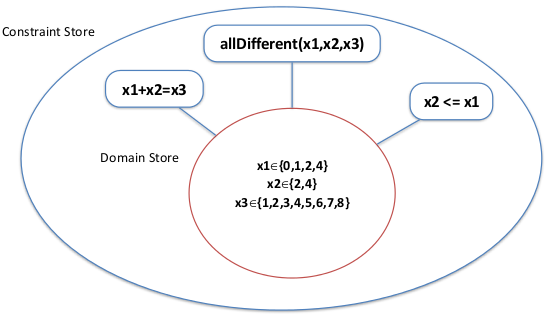
\includegraphics[width=8cm]{fixPoint1}
    & $\Rightarrow$ &
    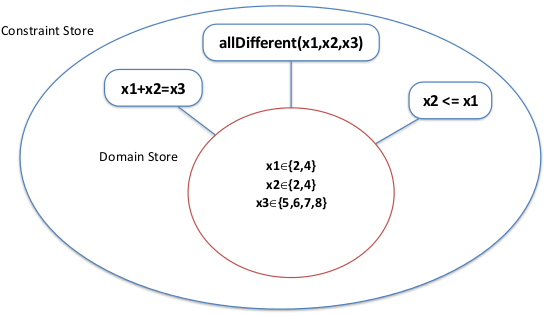
\includegraphics[width=8cm]{fixPoint2}
\end{tabular}


\subsection{Consistency}

\begin{itemize}
    \item A CSP (\textsc{X, D, C}) is $X_{Consistent}$ iff all
        constraints $c \in C$ are $X_{Consistent}$ ($X_{Consistent}$ is
        GAC, BC,\ldots)

    \item A consistency $S_1$ is stronger than a consistency $S_2$ iff all CSP respecting
        $S_1$ also respect $S_2$.

        Note that some consistencies can be \textit{incomparable}

        \begin{center}
            \begin{tabular}{l|c|c|}
                \cline{2-3}
                \multirow{1}{*}{
                    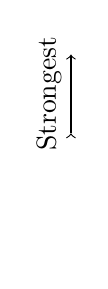
\begin{tikzpicture}
                        \node (0,0) {};
                        \draw[->] (0,1.5) edge node [left]{\rotatebox{90}{Strongest}}
                        (0, 2.5);
                \end{tikzpicture}} 
                &
                \multicolumn{2}{c|}{GAC} \\
                \cline{2-3}
                & Bound consistency & Forward checking \\
                \cline{2-3}
            \end{tabular}
        \end{center}

        This is a tradeoff between \textbf{Speed} and \textbf{Filtering}.

\end{itemize}


\subsubsection{Filtering consistencies}

if $x$ is a domain filtering consistency, a propagator for $x$ will :
from CSP(X, D, X)
\begin{itemize}
    \item return (X, D', C) such that
        \begin{itemize}
            \item D' $\subseteq$ D
            \item (X, D, C) and (X, D', C) equivalent
            \item D' is a nonempty partial solution
            \item (X, D', C) respect $x$
        \end{itemize}
    \item return \textcolor{red}{fail} if no such CSP exists.

        $\to$ not possible to satisfy consistency = unsatisfiable CSP
\end{itemize}

\begin{itemize}
    \item \textbf{Arc consistency} (also called domain consistency):
        every value of every variable participates in a solution of the
        constraint, so all value of variables are \textbf{supported}.

        \begin{tabular}{m{1cm}m{13cm}}
            Note:&
        \begin{itemize}
            \item It's the strongest filtering when considering constraints in isolation.
                \item  GAC $\neq$ satisifability :i A CSP that is GAC may not
        be satisfiable.
        \end{itemize}
        \end{tabular}

        \paragraph{GAC} A constraint $c$ is GAC iff
        \begin{lstlisting}[mathescape]
$\forall x_i \in scope(c)$
    $\forall a_i \in D(x_i)$
        $\exists a_1,..., a_{i-1}, a_{i+1},..., a_r \in D(x_1) \times ... \times D(x_{i-1}) \times D(x_{i+1}) \times ... \times D(x_r)$ such that $(a_1,...,a_r) \in c$
        \end{lstlisting}


    \item \textbf{Bound consistency}: assuming domains are intervals,
        every bound of every variable participates in a solution of the
        constraint.

        \begin{itemize}
            \item GAC can be costly, so a other consistency is to
                only search support for bound.
            \item[$\to$] all valuyes between min and max considered in the domain.
        \end{itemize}


        \paragraph{BC} A constraint $c$ is BC iff
        \begin{lstlisting}[mathescape]
$\forall x_i \in scope(c)$
    $\forall a_i \in \{ \quad min(D(x_i)), max(D(x_i))\quad \}$
        $\exists a_1,..., a_{i-1}, a_{i+1},..., a_r  \in D*(x_1) \times ... \times D*(x_{i-1}) \times D*(x_{i+1}) \times ... \times D*(x_r):$ such that $c(a_1,..., a_r)$

$D*(x_k) = [min(D(x_k)), max(D(x_k))]$
        \end{lstlisting}


    \item \textbf{Forward checking}

        It's like a GAC at the end.

        \paragraph{FC} A constraint $c$ is FC iff
        \begin{lstlisting}[mathescape]
if $\forall x_i \in scope(c):$ $D(x_i) = \{v_i\}$ then $c(v_1, ..., v_r)$
if all but one variable assigned: $c$ is GAC
        \end{lstlisting}
\end{itemize}



\subsection{Global constraints}

\paragraph{Advantage}
\begin{itemize}
    \item Increasing expressivity of CP
    \item Pruning strength because the propagation considered constraint in isolation
        but global constraint is like \textbf{a set of constraint}
    \item Pruning efficiency because no fixed point between small constraints
        but a more flobal reasoning
\end{itemize}

\subsubsection{Decomposition}
A set of constraints $S$ is called the decomposition of $g$ iff :
$$ \forall D(X): sols(X, D(X), \{g\}) = sols(X, D(X), S)$$

\begin{itemize}
    \item GAC pruning equivalent in $S$ and $g$ iff the constraint
        graph of the D is \textbf{acyclic}.

        Otherwise, GAC pruning stronger in global constraint

        \begin{itemize}
            \item GAC on decomposition : supports(s) for each literal on each constraints
                \textbf{separately}
            \item GAC on global constraint: global support(s) for each literal on global constraint
        \end{itemize}


    \item FC pruning stronger in the decomposition
\end{itemize}


\subsubsection{Sum constraint}
\begin{center}
    \texttt{Sum($x_1 + x_2 + ... + x_n$) = K}
\end{center}

\begin{itemize}
    \item \textbf{GAC} for sum constraint is NP-Hard.

        Proof: reduction of subset-sum to GAC for Sum
        \begin{itemize}
            \item subset-sum: a NP-Hard problem for integer set ($S=\{a_1,\cdots, a_r\}$),
                does any non-empty subset of S sums to 0?

            \item reduction to GAC for Sum:
                \begin{lstlisting}[mathescape]
variables  $x_i$ with domains $\{0, a_i\}$
GAC on sum($[x_1,..., x_r], 0$)

if $D(x_i) = \{0\} \forall x_i$ : answer no
else: answer yes
                \end{lstlisting}
        \end{itemize}

       GAC propagator for sum constraint is exponential (unless P=NP).

   \item \textbf{Bound consistency} can be done in $O(n)$

       \begin{lstlisting}[mathescape]
$x_i^{max} = K \sum_{j \neq i} - x_j^{min}$
$x_i^{min} = K \sum_{j \neq i} - x_j^{max}$
       \end{lstlisting}
\end{itemize}

\subsubsection{AllDifferent constraint}
\begin{center}
    \texttt{allDifferent($x_1, x_2,..., x_n$)}
\end{center}

\begin{enumerate}
    \item Build the variable-value graph 

        \begin{tabular}{m{8cm}m{6cm}}
            \begin{itemize}
                \item one node for each variable $x_1,\cdots, x_r$
                \item one node for each value in $\cap D(x_i)$
                \item one edge between $x_i$ and $a$ if $a \in D(x_i)$
                \item[Note:] bipartite graph
            \end{itemize}
            &
            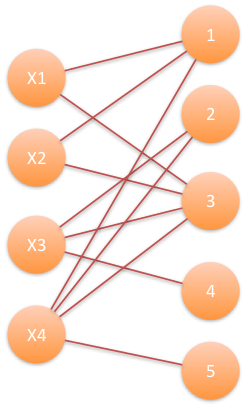
\includegraphics[width=2cm]{variableValue}
        \end{tabular}

    \item There is a solution to allDifferent($x_1, x_2, ..., x_n$)
        if there is a maximum matching of size $n$ in the graph.

        \begin{itemize}
            \item A matching is a \textbf{set of edgges} such that
                no edge share a same node. 
            \item Size matching = \# edges, the maximum size = \#
                variables
        \end{itemize}


        \paragraph{Finding a maximum matching}

        \begin{enumerate}
            \item Start with any matching (e.g. empty matching)
            \item Iteratively improve the matching with \textbf{augmenting path}
                until no more augmenting paths.

                \paragraph{Augmenting path}
                \begin{itemize}
                    \item Edge in M : variables $\to$ values
                    \item Other : values $\to$ variables

                    \item[$\Rightarrow$] An augmenting path is a \textbf{directed path}
                        from a uncovered value to an uncovered variable.
                        Use DSF or BFS
                \end{itemize}

                \begin{figure}[!h]
                    \centering
                    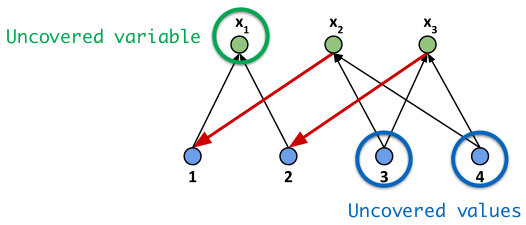
\includegraphics[width=8cm]{augmenting-paths.png}
                    \caption{Augmenting paths}
                \end{figure}

        \end{enumerate}

    \item Remove useless edge by using a \textbf{transformed var-value
        graph} in order to keep edge where there is a directed
        cycle in the transformed graph:
        \begin{itemize}
            \item Alternating path: change value of variable
            \item Alternating cycle: exchange value of variable
        \end{itemize}

        Note that to have the alternate matching, only switch the
        edges in/out.

        \begin{center}
            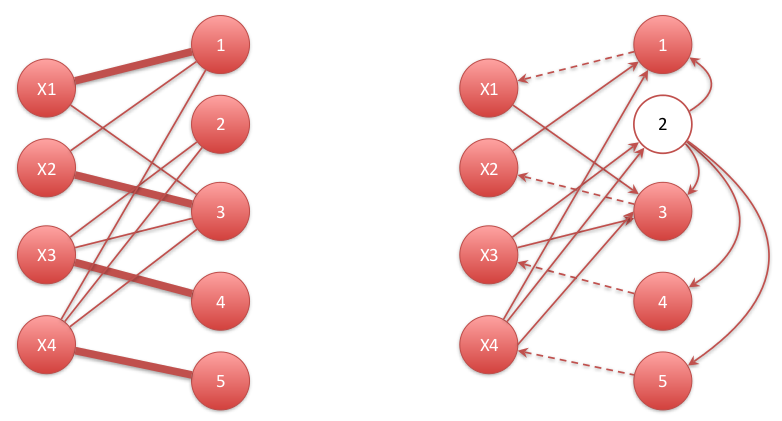
\includegraphics[width=5cm]{transformed}
        \end{center}

        \paragraph{Remove edge}
        Remove all edge $(x, a)$ such that 
        \begin{itemize}
            \item $(x, a)$ is not in the matching 
            \item $a$ and $x$ are in two different Strongly
                Connected Components in the transformed graph because
                there is no directed cycle 
        \end{itemize}

        %TODO show how to make SCC

\end{enumerate}


\subsubsection{Element constraint}

\begin{tabular}{m{6cm}m{6cm}}
    \texttt{Element($c, y$) = x}
    \begin{itemize}
        \item $X = C[Y]$
    \end{itemize}
    &
    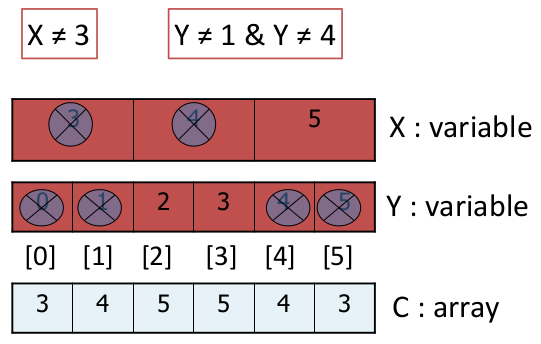
\includegraphics[width=6cm]{elements}
\end{tabular}

\subsubsection{Knapsack constraint}
\begin{center}
    \texttt{binaryKnapsack($x=[0, 1, 0], p=[100, 200, 300], w=[1, 5, 3],
    P=400, W=6$)}
\end{center}
Maximize profit while satisfying the capacity.

\subsubsection{BinPacking constraint}
\begin{center}
    \texttt{binPacking($x=[0, 3, 1], w=[1, 5, 3], l=[4, 0, 6]$)}
\end{center}
Placement of weighted items into capacitated bins.

\subsubsection{Hamiltonian circuit constraint}
\begin{center}
    \texttt{circuit($x[CPIntVar]$)}
\end{center}

\begin{tabular}{m{5cm}m{10cm}}
$x(i)$ is visited after $i$
&
    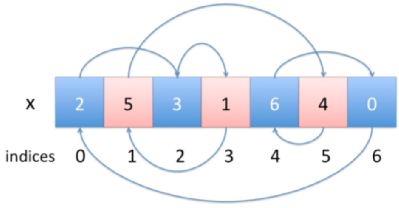
\includegraphics[width=6cm]{hamilto}
\end{tabular}


\subsection{Search}
\begin{itemize}
    \item Recursive search (divide and conquer) with DFS.
        
        The tree is construct during exploration and only the current
        node in memory (DFS). The alternative decisions is memorized.

    \item Branching and variable/value heuristic
        in order to specify for each child nodes
        how to split problem.

        \paragraph{Node expansion}
        Subdivision of a CSP into smaller CSP such that the union of the small CSP
        is equivalent to the original.

\end{itemize}

\subsubsection{Depth First Backtraking search}

\begin{itemize}
    \item Based on:
    \begin{enumerate}
            \item \textbf{stack of sets of decision}
            \item \textbf{stack of restoration states}
        \end{enumerate}
    \item Backtracking restores:
        \begin{enumerate}
            \item Variables/domains
            \item Constraints
            \item Backtracked structures (ex: fistSupport)
        \end{enumerate}
\end{itemize}

\begin{lstlisting}[caption=Depth First backtracking search]
while (! decisionStack.isEmpty) {
    val decisionsOfNode = decisionStack.pop()

    val decision = decisionsOfNode.pop()
    if( decision.hasNext() )
        pushState()

    applyDecision(decision)

    if (!isFailed() ){
        val isExpandable = expand(branching)
        if (! isExpandable) {
            solFound()
            popState()
        }
    } else {
        popState()
    }
}
\end{lstlisting}


\subsubsection{Branching}

\begin{itemize}
    \item A branching strategy is \textbf{completeness}
        if the union of the child CSPs is the parent CSP.

    \item \textbf{Strategy}: 
        \begin{tabular}{l}
            binary labelling ($x_1=a, x_1 \neq a$),\\
            n-ary labelling ($x_1=a, x_1=b, x_1=c, x_1=d$),\\
            domain spliting ($x_1\geq t, x_1 < t$)
        \end{tabular}

    \item \textbf{Variable heuristic}: 
        \begin{tabular}{l}
            Random, lexicographic \\
            Highest number of constraint, variable with unstable
            domain
        \end{tabular}

        \paragraph{First fail principle}: choose first a variable that
        is more likely to fail (Consider the most difficult parts of the
        CSP first).

    \item \textbf{Value heuristic}:
        \begin{tabular}{l}
            Random, lexicographic\\
            Value with minimum pruning, maximum number of solution\\
        \end{tabular}

        \paragraph{Best first principle}: Choose first a value that is
        more likely to succeed
\end{itemize}

\subsubsection{Trailing: restoring state}

\begin{tabular}{m{10cm}m{6cm}}
    In opposition to copying the node in order to perform backtracking,
    trailing only store the \textbf{modification}.

    \begin{itemize}
        \item \textbf{Trail level}
            Trailed operations are marked with an integer which is increase!

        \item \textbf{Restoring} undo all operations with trail level greater than
            desired set the trail level to desired one.
    \end{itemize}

    Sparse set are use to store the domain!
    &
    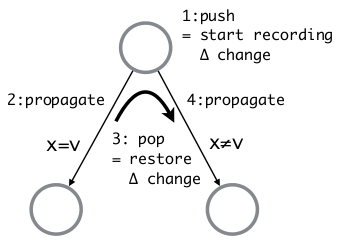
\includegraphics[width=6cm]{trailing}
\end{tabular}

\paragraph{Sparse set data structure}:


\begin{tabular}{m{7cm}m{1.5cm}}
\begin{itemize}
        \item Composed of two table: $dom$ and $map$
        \item $dom$ is split in two set: value in the domain
            are before \textbf{size} and removed value after.

        \item \textbf{}{Invariant} :
            $$ D = \{dom[i] | 0 \leq i \leq size\}$$
            $$map[v] = i \Leftrightarrow dom[i] = v$$
    \end{itemize}
&
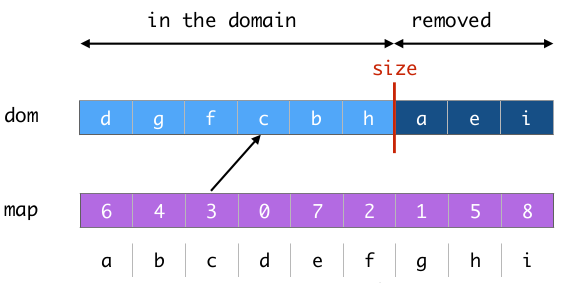
\includegraphics[width=9cm]{sparse.png}
\end{tabular}

\begin{itemize}
    \item \textbf{Checking} if $v$ in the domain: $O(1)$
        \begin{enumerate}
        \item $v \in D \Leftrightarrow map[v] < size$
            \end{enumerate}

    \item \textbf{Removing value} $c$: $O(1)$
        \begin{enumerate}
        \item Exchange value of $map[c]$  and  $map[dom[size-1]$
                \item Decrement $size$ value
            \end{enumerate}

        \item \textbf{Restore removed value}: $0(1)$ thanks to
            ReversibleInteger.

            Note that value are restore in different positions

    \item \textbf{Min/Max} can be added to sparse-set to perform
        efficient BC filtering. 

        When min value are removed, then consider min+1, min+2,...
        until a value in the domain is found (in practive only few
        iterations)

    \item Domain \textbf{iterator} is the only limitation of sparse-set
\end{itemize}



\subsection{Exam}
\begin{itemize}
    \item  Understand how CP works : domain store, fix-point
        algorithm, (reversible) domain implementation.
    \item  Search and First-Fail principle
    \item  Be able to model using element, allDifferent, sum, etc
    \item  Understand Bound-Consistency and Domain
        consistency
    \item  Understand the filtering algorithms for allDifferent, sum,
        etc and be able to design simple filtering algorithms.
\end{itemize}


